% Options for packages loaded elsewhere
\PassOptionsToPackage{unicode}{hyperref}
\PassOptionsToPackage{hyphens}{url}
\PassOptionsToPackage{dvipsnames,svgnames,x11names}{xcolor}
%
\documentclass[
  letterpaper,
]{article}

\usepackage{amsmath,amssymb}
\usepackage{iftex}
\ifPDFTeX
  \usepackage[T1]{fontenc}
  \usepackage[utf8]{inputenc}
  \usepackage{textcomp} % provide euro and other symbols
\else % if luatex or xetex
  \usepackage{unicode-math}
  \defaultfontfeatures{Scale=MatchLowercase}
  \defaultfontfeatures[\rmfamily]{Ligatures=TeX,Scale=1}
\fi
\usepackage{lmodern}
\ifPDFTeX\else  
    % xetex/luatex font selection
\fi
% Use upquote if available, for straight quotes in verbatim environments
\IfFileExists{upquote.sty}{\usepackage{upquote}}{}
\IfFileExists{microtype.sty}{% use microtype if available
  \usepackage[]{microtype}
  \UseMicrotypeSet[protrusion]{basicmath} % disable protrusion for tt fonts
}{}
\makeatletter
\@ifundefined{KOMAClassName}{% if non-KOMA class
  \IfFileExists{parskip.sty}{%
    \usepackage{parskip}
  }{% else
    \setlength{\parindent}{0pt}
    \setlength{\parskip}{6pt plus 2pt minus 1pt}}
}{% if KOMA class
  \KOMAoptions{parskip=half}}
\makeatother
\usepackage{xcolor}
\setlength{\emergencystretch}{3em} % prevent overfull lines
\setcounter{secnumdepth}{-\maxdimen} % remove section numbering
% Make \paragraph and \subparagraph free-standing
\ifx\paragraph\undefined\else
  \let\oldparagraph\paragraph
  \renewcommand{\paragraph}[1]{\oldparagraph{#1}\mbox{}}
\fi
\ifx\subparagraph\undefined\else
  \let\oldsubparagraph\subparagraph
  \renewcommand{\subparagraph}[1]{\oldsubparagraph{#1}\mbox{}}
\fi

\usepackage{color}
\usepackage{fancyvrb}
\newcommand{\VerbBar}{|}
\newcommand{\VERB}{\Verb[commandchars=\\\{\}]}
\DefineVerbatimEnvironment{Highlighting}{Verbatim}{commandchars=\\\{\}}
% Add ',fontsize=\small' for more characters per line
\usepackage{framed}
\definecolor{shadecolor}{RGB}{241,243,245}
\newenvironment{Shaded}{\begin{snugshade}}{\end{snugshade}}
\newcommand{\AlertTok}[1]{\textcolor[rgb]{0.68,0.00,0.00}{#1}}
\newcommand{\AnnotationTok}[1]{\textcolor[rgb]{0.37,0.37,0.37}{#1}}
\newcommand{\AttributeTok}[1]{\textcolor[rgb]{0.40,0.45,0.13}{#1}}
\newcommand{\BaseNTok}[1]{\textcolor[rgb]{0.68,0.00,0.00}{#1}}
\newcommand{\BuiltInTok}[1]{\textcolor[rgb]{0.00,0.23,0.31}{#1}}
\newcommand{\CharTok}[1]{\textcolor[rgb]{0.13,0.47,0.30}{#1}}
\newcommand{\CommentTok}[1]{\textcolor[rgb]{0.37,0.37,0.37}{#1}}
\newcommand{\CommentVarTok}[1]{\textcolor[rgb]{0.37,0.37,0.37}{\textit{#1}}}
\newcommand{\ConstantTok}[1]{\textcolor[rgb]{0.56,0.35,0.01}{#1}}
\newcommand{\ControlFlowTok}[1]{\textcolor[rgb]{0.00,0.23,0.31}{#1}}
\newcommand{\DataTypeTok}[1]{\textcolor[rgb]{0.68,0.00,0.00}{#1}}
\newcommand{\DecValTok}[1]{\textcolor[rgb]{0.68,0.00,0.00}{#1}}
\newcommand{\DocumentationTok}[1]{\textcolor[rgb]{0.37,0.37,0.37}{\textit{#1}}}
\newcommand{\ErrorTok}[1]{\textcolor[rgb]{0.68,0.00,0.00}{#1}}
\newcommand{\ExtensionTok}[1]{\textcolor[rgb]{0.00,0.23,0.31}{#1}}
\newcommand{\FloatTok}[1]{\textcolor[rgb]{0.68,0.00,0.00}{#1}}
\newcommand{\FunctionTok}[1]{\textcolor[rgb]{0.28,0.35,0.67}{#1}}
\newcommand{\ImportTok}[1]{\textcolor[rgb]{0.00,0.46,0.62}{#1}}
\newcommand{\InformationTok}[1]{\textcolor[rgb]{0.37,0.37,0.37}{#1}}
\newcommand{\KeywordTok}[1]{\textcolor[rgb]{0.00,0.23,0.31}{#1}}
\newcommand{\NormalTok}[1]{\textcolor[rgb]{0.00,0.23,0.31}{#1}}
\newcommand{\OperatorTok}[1]{\textcolor[rgb]{0.37,0.37,0.37}{#1}}
\newcommand{\OtherTok}[1]{\textcolor[rgb]{0.00,0.23,0.31}{#1}}
\newcommand{\PreprocessorTok}[1]{\textcolor[rgb]{0.68,0.00,0.00}{#1}}
\newcommand{\RegionMarkerTok}[1]{\textcolor[rgb]{0.00,0.23,0.31}{#1}}
\newcommand{\SpecialCharTok}[1]{\textcolor[rgb]{0.37,0.37,0.37}{#1}}
\newcommand{\SpecialStringTok}[1]{\textcolor[rgb]{0.13,0.47,0.30}{#1}}
\newcommand{\StringTok}[1]{\textcolor[rgb]{0.13,0.47,0.30}{#1}}
\newcommand{\VariableTok}[1]{\textcolor[rgb]{0.07,0.07,0.07}{#1}}
\newcommand{\VerbatimStringTok}[1]{\textcolor[rgb]{0.13,0.47,0.30}{#1}}
\newcommand{\WarningTok}[1]{\textcolor[rgb]{0.37,0.37,0.37}{\textit{#1}}}

\providecommand{\tightlist}{%
  \setlength{\itemsep}{0pt}\setlength{\parskip}{0pt}}\usepackage{longtable,booktabs,array}
\usepackage{calc} % for calculating minipage widths
% Correct order of tables after \paragraph or \subparagraph
\usepackage{etoolbox}
\makeatletter
\patchcmd\longtable{\par}{\if@noskipsec\mbox{}\fi\par}{}{}
\makeatother
% Allow footnotes in longtable head/foot
\IfFileExists{footnotehyper.sty}{\usepackage{footnotehyper}}{\usepackage{footnote}}
\makesavenoteenv{longtable}
\usepackage{graphicx}
\makeatletter
\def\maxwidth{\ifdim\Gin@nat@width>\linewidth\linewidth\else\Gin@nat@width\fi}
\def\maxheight{\ifdim\Gin@nat@height>\textheight\textheight\else\Gin@nat@height\fi}
\makeatother
% Scale images if necessary, so that they will not overflow the page
% margins by default, and it is still possible to overwrite the defaults
% using explicit options in \includegraphics[width, height, ...]{}
\setkeys{Gin}{width=\maxwidth,height=\maxheight,keepaspectratio}
% Set default figure placement to htbp
\makeatletter
\def\fps@figure{htbp}
\makeatother

\makeatletter
\@ifpackageloaded{caption}{}{\usepackage{caption}}
\AtBeginDocument{%
\ifdefined\contentsname
  \renewcommand*\contentsname{Table of contents}
\else
  \newcommand\contentsname{Table of contents}
\fi
\ifdefined\listfigurename
  \renewcommand*\listfigurename{List of Figures}
\else
  \newcommand\listfigurename{List of Figures}
\fi
\ifdefined\listtablename
  \renewcommand*\listtablename{List of Tables}
\else
  \newcommand\listtablename{List of Tables}
\fi
\ifdefined\figurename
  \renewcommand*\figurename{Figure}
\else
  \newcommand\figurename{Figure}
\fi
\ifdefined\tablename
  \renewcommand*\tablename{Table}
\else
  \newcommand\tablename{Table}
\fi
}
\@ifpackageloaded{float}{}{\usepackage{float}}
\floatstyle{ruled}
\@ifundefined{c@chapter}{\newfloat{codelisting}{h}{lop}}{\newfloat{codelisting}{h}{lop}[chapter]}
\floatname{codelisting}{Listing}
\newcommand*\listoflistings{\listof{codelisting}{List of Listings}}
\makeatother
\makeatletter
\makeatother
\makeatletter
\@ifpackageloaded{caption}{}{\usepackage{caption}}
\@ifpackageloaded{subcaption}{}{\usepackage{subcaption}}
\makeatother
\ifLuaTeX
  \usepackage{selnolig}  % disable illegal ligatures
\fi
\usepackage{bookmark}

\IfFileExists{xurl.sty}{\usepackage{xurl}}{} % add URL line breaks if available
\urlstyle{same} % disable monospaced font for URLs
\hypersetup{
  pdftitle={MVP 2},
  pdfauthor={Matt Braaksma},
  colorlinks=true,
  linkcolor={blue},
  filecolor={Maroon},
  citecolor={Blue},
  urlcolor={Blue},
  pdfcreator={LaTeX via pandoc}}

\title{MVP 2}
\usepackage{etoolbox}
\makeatletter
\providecommand{\subtitle}[1]{% add subtitle to \maketitle
  \apptocmd{\@title}{\par {\large #1 \par}}{}{}
}
\makeatother
\subtitle{Advanced Geocomputation}
\author{Matt Braaksma}
\date{}

\begin{document}
\maketitle

\renewcommand*\contentsname{Table of contents}
{
\hypersetup{linkcolor=}
\setcounter{tocdepth}{3}
\tableofcontents
}
\section{Predicting Land Supply
Elasticities}\label{predicting-land-supply-elasticities}

\subsection{Description}\label{description}

Deforestation and cropland expansion are significant global challenges,
contributing to issues such as greenhouse gas emissions and biodiversity
loss. These land-use changes are largely influenced by land supply
elasticities, which measure how responsive land expansion is to price
changes. However, in developing countries where price data is often
unavailable, estimating these elasticities becomes difficult. Villoria
and Liu (2018) address this gap by estimating gridded land supply
elasticities based on factors like market access and land suitability.
This Minimum Viable Product (MVP) focuses on developing an alternative
framework to predict land supply elasticities with the aim of comparing
the econometric model predictions to the machine learning predictions.

The key tasks for this MVP include:

\begin{itemize}
\tightlist
\item
  Gather the raster data from Villoria and Liu (2018)
\item
  Reproject and resample the raster data
\item
  Generate the outcome data from Graesser et al.~(2015)
\item
  Rasterize the outcome data
\item
  Find a suitable sample for the CNN model

  \begin{itemize}
  \tightlist
  \item
    Look for a small square with no missing values
  \end{itemize}
\item
  Combine the predictive rasters into a raster stack
\item
  Build a CNN to predict land elasticities
\end{itemize}

\subsection{Code}\label{code}

\subsubsection{1. Import modules}\label{import-modules}

Import the necessary data, geospatial, visualization modules.

\begin{Shaded}
\begin{Highlighting}[]
\CommentTok{\# Standard Library Imports}
\ImportTok{import}\NormalTok{ os}
\ImportTok{import}\NormalTok{ numpy }\ImportTok{as}\NormalTok{ np}

\CommentTok{\# Data Visualization Imports}
\ImportTok{import}\NormalTok{ matplotlib.pyplot }\ImportTok{as}\NormalTok{ plt}

\CommentTok{\# Geospatial Data Imports}
\ImportTok{from}\NormalTok{ osgeo }\ImportTok{import}\NormalTok{ gdal}
\ImportTok{import}\NormalTok{ geopandas }\ImportTok{as}\NormalTok{ gpd}
\ImportTok{import}\NormalTok{ rasterio}
\ImportTok{from}\NormalTok{ rasterio.features }\ImportTok{import}\NormalTok{ rasterize}

\CommentTok{\# Machine Learning Imports}
\ImportTok{import}\NormalTok{ tensorflow }\ImportTok{as}\NormalTok{ tf}
\ImportTok{from}\NormalTok{ sklearn.model\_selection }\ImportTok{import}\NormalTok{ train\_test\_split}

\CommentTok{\# Set dir}
\CommentTok{\# Define the path to your working directory}
\NormalTok{data\_dir }\OperatorTok{=} \StringTok{\textquotesingle{}../../../base\_data/advgeocomp2024/mvp02\textquotesingle{}}
\NormalTok{data\_dir\_land\_supply }\OperatorTok{=} \StringTok{\textquotesingle{}../../../base\_data/land\_supply\textquotesingle{}}
\NormalTok{os.makedirs(data\_dir, exist\_ok}\OperatorTok{=}\VariableTok{True}\NormalTok{)}
\end{Highlighting}
\end{Shaded}

\subsubsection{2a. Raster Data}\label{a.-raster-data}

\begin{Shaded}
\begin{Highlighting}[]
\CommentTok{\# Raster paths}
\NormalTok{base\_raster\_paths }\OperatorTok{=}\NormalTok{ [}
\NormalTok{    os.path.join(data\_dir\_land\_supply, }\StringTok{\textquotesingle{}anntotprecip/anntotprecip\textquotesingle{}}\NormalTok{),}
\NormalTok{    os.path.join(data\_dir\_land\_supply, }\StringTok{\textquotesingle{}builtupland/builtupland\textquotesingle{}}\NormalTok{),}
\NormalTok{    os.path.join(data\_dir\_land\_supply, }\StringTok{\textquotesingle{}elevation/elevation\textquotesingle{}}\NormalTok{),}
\NormalTok{    os.path.join(data\_dir\_land\_supply, }\StringTok{\textquotesingle{}gl{-}croplands{-}geotif/cropland.tif\textquotesingle{}}\NormalTok{),}
\NormalTok{    os.path.join(data\_dir\_land\_supply, }\StringTok{\textquotesingle{}HWSD2\_RASTER/HWSD2.bil\textquotesingle{}}\NormalTok{),}
\NormalTok{    os.path.join(data\_dir\_land\_supply, }\StringTok{\textquotesingle{}irragland/irragland\textquotesingle{}}\NormalTok{),}
\NormalTok{    os.path.join(data\_dir\_land\_supply, }\StringTok{\textquotesingle{}minutes\_to\_market/minutes\_to\_market\_10s.tif\textquotesingle{}}\NormalTok{), }\CommentTok{\# replacement market access file}
\NormalTok{    os.path.join(data\_dir\_land\_supply, }\StringTok{\textquotesingle{}potentialveg/potveg\textquotesingle{}}\NormalTok{),}
\NormalTok{    os.path.join(data\_dir\_land\_supply, }\StringTok{\textquotesingle{}soilcarbon/soilcarbon\textquotesingle{}}\NormalTok{),}
\NormalTok{    os.path.join(data\_dir\_land\_supply, }\StringTok{\textquotesingle{}SOILPH/soilph\textquotesingle{}}\NormalTok{)}
\NormalTok{]}

\CommentTok{\# Corresponding target paths}
\NormalTok{target\_raster\_paths }\OperatorTok{=}\NormalTok{ [}
\NormalTok{    os.path.join(data\_dir\_land\_supply, }\StringTok{\textquotesingle{}aligned/anntotprecip.tif\textquotesingle{}}\NormalTok{),}
\NormalTok{    os.path.join(data\_dir\_land\_supply, }\StringTok{\textquotesingle{}aligned/builtupland.tif\textquotesingle{}}\NormalTok{),}
\NormalTok{    os.path.join(data\_dir\_land\_supply, }\StringTok{\textquotesingle{}aligned/elevation.tif\textquotesingle{}}\NormalTok{),}
\NormalTok{    os.path.join(data\_dir\_land\_supply, }\StringTok{\textquotesingle{}aligned/cropland.tif\textquotesingle{}}\NormalTok{),}
\NormalTok{    os.path.join(data\_dir\_land\_supply, }\StringTok{\textquotesingle{}aligned/HWSD2.tif\textquotesingle{}}\NormalTok{),}
\NormalTok{    os.path.join(data\_dir\_land\_supply, }\StringTok{\textquotesingle{}aligned/irragland.tif\textquotesingle{}}\NormalTok{),}
\NormalTok{    os.path.join(data\_dir\_land\_supply, }\StringTok{\textquotesingle{}aligned/minutes\_to\_market\_10s.tif\textquotesingle{}}\NormalTok{),}
\NormalTok{    os.path.join(data\_dir\_land\_supply, }\StringTok{\textquotesingle{}aligned/potentialveg.tif\textquotesingle{}}\NormalTok{),}
\NormalTok{    os.path.join(data\_dir\_land\_supply, }\StringTok{\textquotesingle{}aligned/soilcarbon.tif\textquotesingle{}}\NormalTok{),}
\NormalTok{    os.path.join(data\_dir\_land\_supply, }\StringTok{\textquotesingle{}aligned/SOILPH.tif\textquotesingle{}}\NormalTok{)}
\NormalTok{]}

\CommentTok{\# Create the target directory if it doesn\textquotesingle{}t exist}
\ControlFlowTok{if} \KeywordTok{not}\NormalTok{ os.path.exists(os.path.join(data\_dir\_land\_supply, }\StringTok{\textquotesingle{}aligned\textquotesingle{}}\NormalTok{)):}
\NormalTok{    os.mkdir(os.path.join(data\_dir\_land\_supply, }\StringTok{\textquotesingle{}aligned\textquotesingle{}}\NormalTok{))}

\CommentTok{\# Loop through the base rasters and apply the gdal.Warp function}
\ControlFlowTok{for}\NormalTok{ base\_raster\_path, target\_raster\_path }\KeywordTok{in} \BuiltInTok{zip}\NormalTok{(base\_raster\_paths, target\_raster\_paths):     }
    \CommentTok{\# Using gdal.Warp to reproject and resize}
\NormalTok{    gdal.Warp(}
\NormalTok{        target\_raster\_path,}
\NormalTok{        base\_raster\_path,}
\NormalTok{        xRes}\OperatorTok{=}\FloatTok{0.7}\NormalTok{,}
\NormalTok{        yRes}\OperatorTok{=}\FloatTok{0.7}\NormalTok{,}
\NormalTok{        resampleAlg}\OperatorTok{=}\StringTok{\textquotesingle{}bilinear\textquotesingle{}}\NormalTok{,         }
\NormalTok{        dstSRS}\OperatorTok{=}\StringTok{\textquotesingle{}EPSG:4326\textquotesingle{}}  
\NormalTok{    )}
    \BuiltInTok{print}\NormalTok{(}\SpecialStringTok{f"Raster succesfully processed and saved to }\SpecialCharTok{\{}\NormalTok{target\_raster\_path}\SpecialCharTok{\}}\SpecialStringTok{."}\NormalTok{)}
\end{Highlighting}
\end{Shaded}

\begin{verbatim}
Raster succesfully processed and saved to ../../../base_data/land_supply/aligned/anntotprecip.tif.
Raster succesfully processed and saved to ../../../base_data/land_supply/aligned/builtupland.tif.
Raster succesfully processed and saved to ../../../base_data/land_supply/aligned/elevation.tif.
Raster succesfully processed and saved to ../../../base_data/land_supply/aligned/cropland.tif.
Raster succesfully processed and saved to ../../../base_data/land_supply/aligned/HWSD2.tif.
Raster succesfully processed and saved to ../../../base_data/land_supply/aligned/irragland.tif.
Raster succesfully processed and saved to ../../../base_data/land_supply/aligned/minutes_to_market_10s.tif.
Raster succesfully processed and saved to ../../../base_data/land_supply/aligned/potentialveg.tif.
Raster succesfully processed and saved to ../../../base_data/land_supply/aligned/soilcarbon.tif.
Raster succesfully processed and saved to ../../../base_data/land_supply/aligned/SOILPH.tif.
\end{verbatim}

\subsubsection{2b. Vector Data}\label{b.-vector-data}

\begin{Shaded}
\begin{Highlighting}[]
\CommentTok{\# Load shapefile}
\NormalTok{ecos\_path }\OperatorTok{=}\NormalTok{ os.path.join(data\_dir, }\StringTok{\textquotesingle{}TerrestrialEcos\textquotesingle{}}\NormalTok{)}
\NormalTok{gdf }\OperatorTok{=}\NormalTok{ gpd.read\_file(ecos\_path)}

\CommentTok{\# Define the eco\_names and their observed values from the figure in Graesser et al. (2015)}
\NormalTok{eco\_name\_observed\_values }\OperatorTok{=}\NormalTok{ \{}
    \StringTok{\textquotesingle{}Araucaria moist forests\textquotesingle{}}\NormalTok{: }\FloatTok{0.12}\NormalTok{,}
    \StringTok{\textquotesingle{}Alto Paraná Atlantic forests\textquotesingle{}}\NormalTok{: }\FloatTok{0.15}\NormalTok{,}
    \StringTok{\textquotesingle{}Uruguayan savanna\textquotesingle{}}\NormalTok{: }\FloatTok{0.18}\NormalTok{,}
    \StringTok{\textquotesingle{}Llanos\textquotesingle{}}\NormalTok{: }\FloatTok{0.10}\NormalTok{,}
    \StringTok{\textquotesingle{}Espinal\textquotesingle{}}\NormalTok{: }\FloatTok{0.08}\NormalTok{,}
    \StringTok{\textquotesingle{}Humid Pampas\textquotesingle{}}\NormalTok{: }\FloatTok{0.07}\NormalTok{,}
    \StringTok{\textquotesingle{}Humid Chaco\textquotesingle{}}\NormalTok{: }\FloatTok{0.09}\NormalTok{,}
    \StringTok{\textquotesingle{}Peten–Veracruz moist forests\textquotesingle{}}\NormalTok{: }\FloatTok{0.05}\NormalTok{,}
    \StringTok{\textquotesingle{}Chiquitano dry forests\textquotesingle{}}\NormalTok{: }\FloatTok{0.03}\NormalTok{,}
    \StringTok{\textquotesingle{}Dry Chaco\textquotesingle{}}\NormalTok{: }\FloatTok{0.20}\NormalTok{,}
    \StringTok{\textquotesingle{}Cerrado\textquotesingle{}}\NormalTok{: }\FloatTok{0.25}\NormalTok{,}
    \StringTok{\textquotesingle{}Mato Grosso seasonal forests\textquotesingle{}}\NormalTok{: }\FloatTok{0.60}
\NormalTok{\}}

\CommentTok{\# Filter the GeoDataFrame to include only the specified eco\_names}
\NormalTok{subset\_gdf }\OperatorTok{=}\NormalTok{ gdf[gdf[}\StringTok{\textquotesingle{}ECO\_NAME\textquotesingle{}}\NormalTok{].isin(eco\_name\_observed\_values.keys())].copy()}

\CommentTok{\# Add a new column \textquotesingle{}observed\_value\textquotesingle{} with the corresponding observed values}
\NormalTok{subset\_gdf.loc[:, }\StringTok{\textquotesingle{}observed\_value\textquotesingle{}}\NormalTok{] }\OperatorTok{=}\NormalTok{ subset\_gdf[}\StringTok{\textquotesingle{}ECO\_NAME\textquotesingle{}}\NormalTok{].}\BuiltInTok{map}\NormalTok{(eco\_name\_observed\_values)}

\CommentTok{\# Load the template raster file}
\ControlFlowTok{with}\NormalTok{ rasterio.}\BuiltInTok{open}\NormalTok{(target\_raster\_paths[}\DecValTok{0}\NormalTok{]) }\ImportTok{as}\NormalTok{ src:}
\NormalTok{    template\_meta }\OperatorTok{=}\NormalTok{ src.meta.copy()}
\NormalTok{    template\_shape }\OperatorTok{=}\NormalTok{ src.shape}
\NormalTok{    template\_transform }\OperatorTok{=}\NormalTok{ src.transform}

\CommentTok{\# Prepare geometries and values for rasterization}
\CommentTok{\# Each geometry should have its \textquotesingle{}observed\_value\textquotesingle{} mapped to it}
\NormalTok{shapes }\OperatorTok{=}\NormalTok{ ((geom, value) }\ControlFlowTok{for}\NormalTok{ geom, value }\KeywordTok{in} \BuiltInTok{zip}\NormalTok{(subset\_gdf.geometry, subset\_gdf[}\StringTok{\textquotesingle{}observed\_value\textquotesingle{}}\NormalTok{]))}

\CommentTok{\# Rasterize using the template raster\textquotesingle{}s shape and transform}
\NormalTok{rasterized\_data }\OperatorTok{=}\NormalTok{ rasterize(}
\NormalTok{    shapes}\OperatorTok{=}\NormalTok{shapes,}
\NormalTok{    out\_shape}\OperatorTok{=}\NormalTok{template\_shape,}
\NormalTok{    transform}\OperatorTok{=}\NormalTok{template\_transform,}
\NormalTok{    fill}\OperatorTok{=}\DecValTok{0}\NormalTok{,  }\CommentTok{\# background value, e.g., 0 for no data}
\NormalTok{    dtype}\OperatorTok{=}\StringTok{\textquotesingle{}float32\textquotesingle{}}  \CommentTok{\# use a suitable data type}
\NormalTok{)}

\CommentTok{\# Update metadata to match the output raster}
\NormalTok{output\_meta }\OperatorTok{=}\NormalTok{ template\_meta.copy()}
\NormalTok{output\_meta.update(\{}\StringTok{"dtype"}\NormalTok{: }\StringTok{\textquotesingle{}float32\textquotesingle{}}\NormalTok{, }\StringTok{"count"}\NormalTok{: }\DecValTok{1}\NormalTok{\})}

\CommentTok{\# Save the rasterized output to a new file}
\NormalTok{output\_path }\OperatorTok{=}\NormalTok{ os.path.join(data\_dir, }\StringTok{\textquotesingle{}rasterized\_ecos.tif\textquotesingle{}}\NormalTok{)}
\ControlFlowTok{with}\NormalTok{ rasterio.}\BuiltInTok{open}\NormalTok{(output\_path, }\StringTok{\textquotesingle{}w\textquotesingle{}}\NormalTok{, }\OperatorTok{**}\NormalTok{output\_meta) }\ImportTok{as}\NormalTok{ dst:}
\NormalTok{    dst.write(rasterized\_data, }\DecValTok{1}\NormalTok{)}
\end{Highlighting}
\end{Shaded}

\subsubsection{3. Build CNN model}\label{build-cnn-model}

data\_dir\_land\_supply

\begin{Shaded}
\begin{Highlighting}[]
\CommentTok{\# Function to load a raster file and return its array representation}
\KeywordTok{def}\NormalTok{ load\_raster(raster\_path):}
    \CommentTok{"""Loads a raster file from the given path and returns it as a NumPy array."""}
\NormalTok{    dataset }\OperatorTok{=}\NormalTok{ gdal.Open(raster\_path)  }\CommentTok{\# Open the raster file}
\NormalTok{    array }\OperatorTok{=}\NormalTok{ dataset.ReadAsArray()     }\CommentTok{\# Read the raster data into a NumPy array}
\NormalTok{    dataset }\OperatorTok{=} \VariableTok{None}
    \ControlFlowTok{return}\NormalTok{ array}

\CommentTok{\# Function to load and stack multiple raster files}
\KeywordTok{def}\NormalTok{ load\_and\_stack\_rasters(raster\_paths):}
    \CommentTok{"""}
\CommentTok{    Loads multiple raster files and stacks them along a new axis for CNN input}
\CommentTok{    (height, width, channels).}
\CommentTok{    """}
\NormalTok{    raster\_stack }\OperatorTok{=}\NormalTok{ []  }\CommentTok{\# List to store individual raster arrays}
    
    \CommentTok{\# Loop through each raster path, load the raster, and append it to the list}
    \ControlFlowTok{for}\NormalTok{ path }\KeywordTok{in}\NormalTok{ raster\_paths:}
\NormalTok{        array }\OperatorTok{=}\NormalTok{ load\_raster(path)}
\NormalTok{        raster\_stack.append(array)}
        \BuiltInTok{print}\NormalTok{(}\SpecialStringTok{f"Loaded }\SpecialCharTok{\{}\NormalTok{path}\SpecialCharTok{\}}\SpecialStringTok{ with shape }\SpecialCharTok{\{}\NormalTok{array}\SpecialCharTok{.}\NormalTok{shape}\SpecialCharTok{\}}\SpecialStringTok{"}\NormalTok{)}
    
    \CommentTok{\# Stack the loaded rasters along a new axis (creating the \textquotesingle{}channels\textquotesingle{} dimension)}
    \ControlFlowTok{return}\NormalTok{ np.stack(raster\_stack, axis}\OperatorTok{={-}}\DecValTok{1}\NormalTok{)}

\CommentTok{\# Load and stack the rasters}
\NormalTok{raster\_paths }\OperatorTok{=}\NormalTok{ [}
\NormalTok{    os.path.join(data\_dir\_land\_supply, }\StringTok{\textquotesingle{}aligned/anntotprecip.tif\textquotesingle{}}\NormalTok{),}
    \CommentTok{\# os.path.join(data\_dir\_land\_supply, \textquotesingle{}aligned/builtupland.tif\textquotesingle{}), \# Not the same dimensions as the other rasters}
\NormalTok{    os.path.join(data\_dir\_land\_supply, }\StringTok{\textquotesingle{}aligned/elevation.tif\textquotesingle{}}\NormalTok{),}
\NormalTok{    os.path.join(data\_dir\_land\_supply, }\StringTok{\textquotesingle{}aligned/cropland.tif\textquotesingle{}}\NormalTok{),}
\NormalTok{    os.path.join(data\_dir\_land\_supply, }\StringTok{\textquotesingle{}aligned/HWSD2.tif\textquotesingle{}}\NormalTok{),}
\NormalTok{    os.path.join(data\_dir\_land\_supply, }\StringTok{\textquotesingle{}aligned/irragland.tif\textquotesingle{}}\NormalTok{),}
\NormalTok{    os.path.join(data\_dir\_land\_supply, }\StringTok{\textquotesingle{}aligned/minutes\_to\_market\_10s.tif\textquotesingle{}}\NormalTok{),}
\NormalTok{    os.path.join(data\_dir\_land\_supply, }\StringTok{\textquotesingle{}aligned/potentialveg.tif\textquotesingle{}}\NormalTok{),}
\NormalTok{    os.path.join(data\_dir\_land\_supply, }\StringTok{\textquotesingle{}aligned/soilcarbon.tif\textquotesingle{}}\NormalTok{),}
\NormalTok{    os.path.join(data\_dir\_land\_supply, }\StringTok{\textquotesingle{}aligned/SOILPH.tif\textquotesingle{}}\NormalTok{)}
\NormalTok{]}
\NormalTok{raster\_stack }\OperatorTok{=}\NormalTok{ load\_and\_stack\_rasters(raster\_paths)}

\CommentTok{\# Function to find a square area without missing data (zeros) in the outcome raster}
\KeywordTok{def}\NormalTok{ find\_square\_with\_complete\_outcome(outcome\_raster, raster\_stack, square\_size):}
    \CommentTok{"""}
\CommentTok{    Finds a square region in the outcome raster with no zero values,}
\CommentTok{    then extracts the corresponding square region from the raster stack.}
\CommentTok{    """}
\NormalTok{    height, width }\OperatorTok{=}\NormalTok{ outcome\_raster.shape  }\CommentTok{\# Get dimensions of the outcome raster}
\NormalTok{    x\_max\_start }\OperatorTok{=}\NormalTok{ width }\OperatorTok{{-}}\NormalTok{ square\_size     }\CommentTok{\# Maximum starting x{-}coordinate for the square}
\NormalTok{    y\_max\_start }\OperatorTok{=}\NormalTok{ height }\OperatorTok{{-}}\NormalTok{ square\_size    }\CommentTok{\# Maximum starting y{-}coordinate for the square}
    
    \CommentTok{\# Loop through the raster, stepping by the square size}
    \ControlFlowTok{for}\NormalTok{ y\_start }\KeywordTok{in} \BuiltInTok{range}\NormalTok{(}\DecValTok{0}\NormalTok{, y\_max\_start }\OperatorTok{+} \DecValTok{1}\NormalTok{, square\_size):}
        \ControlFlowTok{for}\NormalTok{ x\_start }\KeywordTok{in} \BuiltInTok{range}\NormalTok{(}\DecValTok{0}\NormalTok{, x\_max\_start }\OperatorTok{+} \DecValTok{1}\NormalTok{, square\_size):}
            \CommentTok{\# Extract the square region from the outcome raster}
\NormalTok{            outcome\_square }\OperatorTok{=}\NormalTok{ outcome\_raster[y\_start:y\_start }\OperatorTok{+}\NormalTok{ square\_size, x\_start:x\_start }\OperatorTok{+}\NormalTok{ square\_size]}
            
            \CommentTok{\# Check if there are any missing data (zeros) in the square region}
\NormalTok{            has\_missing\_data }\OperatorTok{=}\NormalTok{ (outcome\_square }\OperatorTok{==} \DecValTok{0}\NormalTok{).}\BuiltInTok{any}\NormalTok{()}
            
            \CommentTok{\# If no missing data, extract the corresponding region from the raster stack}
            \ControlFlowTok{if} \KeywordTok{not}\NormalTok{ has\_missing\_data:}
\NormalTok{                predictor\_square }\OperatorTok{=}\NormalTok{ raster\_stack[y\_start:y\_start }\OperatorTok{+}\NormalTok{ square\_size, x\_start:x\_start }\OperatorTok{+}\NormalTok{ square\_size, :]}
                \ControlFlowTok{return}\NormalTok{ predictor\_square, outcome\_square}
    
    \CommentTok{\# Raise an error if no valid square was found}
    \ControlFlowTok{raise} \PreprocessorTok{ValueError}\NormalTok{(}\StringTok{"No square region without zero values in the outcome raster was found."}\NormalTok{)}

\CommentTok{\# Path to the outcome raster (dependent variable)}
\NormalTok{outcome\_raster\_path }\OperatorTok{=}\NormalTok{ os.path.join(data\_dir, }\StringTok{\textquotesingle{}rasterized\_ecos.tif\textquotesingle{}}\NormalTok{)}

\CommentTok{\# Load the outcome raster}
\NormalTok{outcome\_raster }\OperatorTok{=}\NormalTok{ load\_raster(outcome\_raster\_path)}

\CommentTok{\# Example usage: Find a 12x12 area without zero values in the outcome}
\CommentTok{\# 12 is the largest available square}
\NormalTok{square\_size }\OperatorTok{=} \DecValTok{12}

\ControlFlowTok{try}\NormalTok{:}
    \CommentTok{\# Find a valid square region}
\NormalTok{    predictor\_square, outcome\_square }\OperatorTok{=}\NormalTok{ find\_square\_with\_complete\_outcome(outcome\_raster, raster\_stack, square\_size)}
    \BuiltInTok{print}\NormalTok{(}\StringTok{"Found a valid square area without zero values in the outcome raster."}\NormalTok{)}
    
    \CommentTok{\# Plot the outcome square}
\NormalTok{    plt.figure(figsize}\OperatorTok{=}\NormalTok{(}\DecValTok{10}\NormalTok{, }\DecValTok{8}\NormalTok{))}
\NormalTok{    plt.imshow(outcome\_square, cmap}\OperatorTok{=}\StringTok{\textquotesingle{}viridis\textquotesingle{}}\NormalTok{, vmin}\OperatorTok{=}\NormalTok{np.}\BuiltInTok{min}\NormalTok{(outcome\_raster), vmax}\OperatorTok{=}\NormalTok{np.}\BuiltInTok{max}\NormalTok{(outcome\_raster))}
\NormalTok{    plt.colorbar(label}\OperatorTok{=}\StringTok{\textquotesingle{}Land Supply Elasticity\textquotesingle{}}\NormalTok{)}
\NormalTok{    plt.title(}\StringTok{\textquotesingle{}Outcome Raster (Land Supply Elasticity)\textquotesingle{}}\NormalTok{)}
\NormalTok{    plt.show()}
\ControlFlowTok{except} \PreprocessorTok{ValueError} \ImportTok{as}\NormalTok{ e:}
    \BuiltInTok{print}\NormalTok{(e)}
\end{Highlighting}
\end{Shaded}

\begin{verbatim}
Loaded ../../../base_data/land_supply/aligned/anntotprecip.tif with shape (257, 514)
Loaded ../../../base_data/land_supply/aligned/elevation.tif with shape (257, 514)
Loaded ../../../base_data/land_supply/aligned/cropland.tif with shape (257, 514)
Loaded ../../../base_data/land_supply/aligned/HWSD2.tif with shape (257, 514)
Loaded ../../../base_data/land_supply/aligned/irragland.tif with shape (257, 514)
Loaded ../../../base_data/land_supply/aligned/minutes_to_market_10s.tif with shape (257, 514)
Loaded ../../../base_data/land_supply/aligned/potentialveg.tif with shape (257, 514)
Loaded ../../../base_data/land_supply/aligned/soilcarbon.tif with shape (257, 514)
Loaded ../../../base_data/land_supply/aligned/SOILPH.tif with shape (257, 514)
Found a valid square area without zero values in the outcome raster.
\end{verbatim}

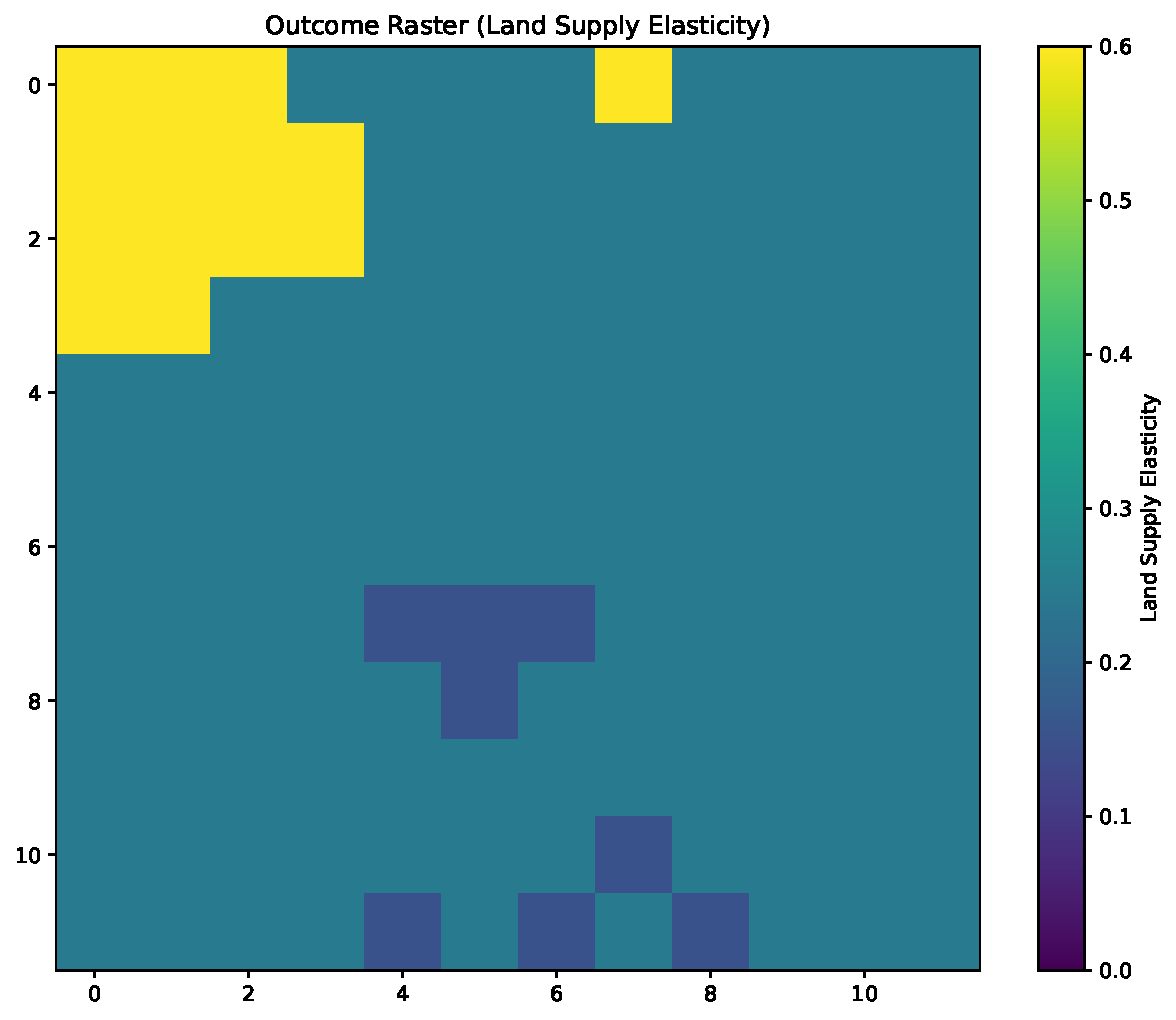
\includegraphics{mvp02_files/figure-pdf/cell-5-output-2.pdf}

\begin{Shaded}
\begin{Highlighting}[]
\CommentTok{\# Assuming \textasciigrave{}predictor\_square\textasciigrave{} and \textasciigrave{}outcome\_square\textasciigrave{} are lists of extracted squares}
\NormalTok{predictor\_squares }\OperatorTok{=}\NormalTok{ np.array(predictor\_square)  }\CommentTok{\# Shape: (num\_samples, square\_size, square\_size, num\_rasters)}
\NormalTok{outcome\_squares }\OperatorTok{=}\NormalTok{ np.array(outcome\_square)      }\CommentTok{\# Shape: (num\_samples, 1)}

\CommentTok{\# Add a channel dimension to predictor\_squares if it\textquotesingle{}s missing}
\NormalTok{predictor\_squares }\OperatorTok{=}\NormalTok{ np.expand\_dims(predictor\_squares, axis}\OperatorTok{={-}}\DecValTok{1}\NormalTok{)  }\CommentTok{\# Adding channel dimension (if needed)}

\CommentTok{\# Split the data into training and test sets}
\NormalTok{X\_train, X\_test, y\_train, y\_test }\OperatorTok{=}\NormalTok{ train\_test\_split(predictor\_squares, outcome\_squares, test\_size}\OperatorTok{=}\FloatTok{0.2}\NormalTok{, random\_state}\OperatorTok{=}\DecValTok{42}\NormalTok{)}

\CommentTok{\# Ensure y\_train is 2D (num\_samples, 1)}
\NormalTok{y\_train }\OperatorTok{=}\NormalTok{ np.expand\_dims(y\_train, axis}\OperatorTok{={-}}\DecValTok{1}\NormalTok{)  }\CommentTok{\# Ensure it\textquotesingle{}s a 2D array (num\_samples, 1)}

\CommentTok{\# Define the CNN model architecture}
\KeywordTok{def}\NormalTok{ build\_cnn\_model(input\_shape):}
\NormalTok{    model }\OperatorTok{=}\NormalTok{ tf.keras.models.Sequential([}
\NormalTok{        tf.keras.layers.Conv2D(}\DecValTok{32}\NormalTok{, (}\DecValTok{3}\NormalTok{, }\DecValTok{3}\NormalTok{), activation}\OperatorTok{=}\StringTok{\textquotesingle{}relu\textquotesingle{}}\NormalTok{, padding}\OperatorTok{=}\StringTok{\textquotesingle{}same\textquotesingle{}}\NormalTok{, input\_shape}\OperatorTok{=}\NormalTok{input\_shape),}
\NormalTok{        tf.keras.layers.MaxPooling2D((}\DecValTok{2}\NormalTok{, }\DecValTok{2}\NormalTok{), padding}\OperatorTok{=}\StringTok{\textquotesingle{}same\textquotesingle{}}\NormalTok{),}
        
\NormalTok{        tf.keras.layers.Conv2D(}\DecValTok{64}\NormalTok{, (}\DecValTok{3}\NormalTok{, }\DecValTok{3}\NormalTok{), activation}\OperatorTok{=}\StringTok{\textquotesingle{}relu\textquotesingle{}}\NormalTok{, padding}\OperatorTok{=}\StringTok{\textquotesingle{}same\textquotesingle{}}\NormalTok{),}
\NormalTok{        tf.keras.layers.MaxPooling2D((}\DecValTok{2}\NormalTok{, }\DecValTok{2}\NormalTok{), padding}\OperatorTok{=}\StringTok{\textquotesingle{}same\textquotesingle{}}\NormalTok{),}
        
\NormalTok{        tf.keras.layers.Conv2D(}\DecValTok{128}\NormalTok{, (}\DecValTok{3}\NormalTok{, }\DecValTok{3}\NormalTok{), activation}\OperatorTok{=}\StringTok{\textquotesingle{}relu\textquotesingle{}}\NormalTok{, padding}\OperatorTok{=}\StringTok{\textquotesingle{}same\textquotesingle{}}\NormalTok{),}
\NormalTok{        tf.keras.layers.GlobalAveragePooling2D(),}
        
\NormalTok{        tf.keras.layers.Dense(}\DecValTok{64}\NormalTok{, activation}\OperatorTok{=}\StringTok{\textquotesingle{}relu\textquotesingle{}}\NormalTok{),}
\NormalTok{        tf.keras.layers.Dense(}\DecValTok{1}\NormalTok{)  }\CommentTok{\# Single output for regression}
\NormalTok{    ])}
    \ControlFlowTok{return}\NormalTok{ model}

\CommentTok{\# Build the model}
\NormalTok{input\_shape }\OperatorTok{=}\NormalTok{ X\_train.shape[}\DecValTok{1}\NormalTok{:]  }\CommentTok{\# (square\_size, square\_size, num\_rasters)}
\NormalTok{model }\OperatorTok{=}\NormalTok{ build\_cnn\_model(input\_shape)}

\CommentTok{\# Compile the model for regression}
\NormalTok{model.}\BuiltInTok{compile}\NormalTok{(optimizer}\OperatorTok{=}\StringTok{\textquotesingle{}adam\textquotesingle{}}\NormalTok{, loss}\OperatorTok{=}\StringTok{\textquotesingle{}mse\textquotesingle{}}\NormalTok{, metrics}\OperatorTok{=}\NormalTok{[}\StringTok{\textquotesingle{}mae\textquotesingle{}}\NormalTok{])}

\CommentTok{\# Train the model}
\NormalTok{epochs }\OperatorTok{=} \DecValTok{4}
\NormalTok{batch\_size }\OperatorTok{=} \DecValTok{16}
\NormalTok{history }\OperatorTok{=}\NormalTok{ model.fit(X\_train, y\_train, epochs}\OperatorTok{=}\NormalTok{epochs, batch\_size}\OperatorTok{=}\NormalTok{batch\_size, validation\_split}\OperatorTok{=}\FloatTok{0.2}\NormalTok{)}

\CommentTok{\# \# Evaluate the model on the test data}
\CommentTok{\# test\_loss, test\_mae = model.evaluate(X\_test, y\_test)}
\CommentTok{\# print(f"Test Mean Absolute Error: \{test\_mae\}")}

\CommentTok{\# \# Predict on new data (example)}
\CommentTok{\# predictions = model.predict(X\_test)}
\end{Highlighting}
\end{Shaded}

\begin{verbatim}
Epoch 1/4
1/1 ━━━━━━━━━━━━━━━━━━━━ 0s 470ms/step - loss: inf - mae: 9051744043519887332757109517102088192.00001/1 ━━━━━━━━━━━━━━━━━━━━ 1s 533ms/step - loss: inf - mae: 9051744043519887332757109517102088192.0000 - val_loss: nan - val_mae: nan
Epoch 2/4
1/1 ━━━━━━━━━━━━━━━━━━━━ 0s 9ms/step - loss: nan - mae: nan1/1 ━━━━━━━━━━━━━━━━━━━━ 0s 19ms/step - loss: nan - mae: nan - val_loss: nan - val_mae: nan
Epoch 3/4
1/1 ━━━━━━━━━━━━━━━━━━━━ 0s 9ms/step - loss: nan - mae: nan1/1 ━━━━━━━━━━━━━━━━━━━━ 0s 18ms/step - loss: nan - mae: nan - val_loss: nan - val_mae: nan
Epoch 4/4
1/1 ━━━━━━━━━━━━━━━━━━━━ 0s 9ms/step - loss: nan - mae: nan1/1 ━━━━━━━━━━━━━━━━━━━━ 0s 18ms/step - loss: nan - mae: nan - val_loss: nan - val_mae: nan
\end{verbatim}

\begin{verbatim}
/Users/mbraaksma/mambaforge/envs/geovenv1/lib/python3.10/site-packages/keras/src/layers/convolutional/base_conv.py:107: UserWarning:

Do not pass an `input_shape`/`input_dim` argument to a layer. When using Sequential models, prefer using an `Input(shape)` object as the first layer in the model instead.
\end{verbatim}

As seen in the final epochs, the CNN fails which means the final
predictions cannot be made. After multiple attempts to address this, I
believe the small outcome raster size is the limiting factor, which is a
significant data limitation.

\subsection{Design Framework}\label{design-framework}

\paragraph{Problem}\label{problem}

How would predictions from a machine learning approach differ from
econometric predictions?

Villoria \& Liu (2018) estimate gridded land supply elasticities using
an econometric specification based on market access and land suitability
factors.

\paragraph{Solution}\label{solution}

Answering this question requires a significant amount of data gathering.
First, the market access and land suitability data from Villoria \& Liu
(2018) must be downloaded. Next, the validation data from Graesser et
al.~(2015) must be found and downloaded. After ensuring that all the
data is a proper format to work nicely together, a sample must be taken
to use for building the machine learning model. A CNN regression model
can be used to predict land supply elasticities. Finally, this can be
compared to the replicated gridded elasticities from Villoria \& Liu
(2018).

\paragraph{Challenge}\label{challenge}

Sourcing the data and ensuring that the different pieces work well
together.

\paragraph{Spec list}\label{spec-list}

\begin{longtable}[]{@{}
  >{\raggedright\arraybackslash}p{(\columnwidth - 4\tabcolsep) * \real{0.3333}}
  >{\raggedright\arraybackslash}p{(\columnwidth - 4\tabcolsep) * \real{0.3333}}
  >{\raggedright\arraybackslash}p{(\columnwidth - 4\tabcolsep) * \real{0.3333}}@{}}
\toprule\noalign{}
\begin{minipage}[b]{\linewidth}\raggedright
Spec
\end{minipage} & \begin{minipage}[b]{\linewidth}\raggedright
Value (H, M, L)
\end{minipage} & \begin{minipage}[b]{\linewidth}\raggedright
Effort (H, M, L)
\end{minipage} \\
\midrule\noalign{}
\endhead
\bottomrule\noalign{}
\endlastfoot
Get data used in Villoria \& Liu (2018) & H & M \\
Get validation data from Graesser et al.~(2015) & H & M \\
Clean Data (align, reproject, etc) & H & M \\
Build CNN to predict land supply elasticities & H & H \\
Replicate Villoria \& Liu (2018) estimates & L & M \\
Compare methods & H & M \\
\end{longtable}

\paragraph{Success}\label{success}

After detailing the steps for this MVP, is it likely that it will not be
possible to complete. A success for this MVP would be to build a CNN
model that can be used for prediction on raster data. My goal is to
learn how to do so in a realistic setting, even if the final result is
incomplete.

\paragraph{Reflection}\label{reflection}

During this MVP, I encountered several significant challenges:

\begin{itemize}
\tightlist
\item
  Data Limitations: The outcome data was not accessible, so I had to
  locate a relevant shapefile and construct the variable based on a
  figure.
\item
  Rasterization Issues: The resulting rasterized outcome contained
  numerous missing values, limiting the largest viable square sample for
  the CNN model to only 12x12 pixels. I wasn't sure of alternative
  approaches for handling missing outcome data.
\item
  Model Constraints: The limited sample size seemed insufficient for the
  CNN. Although the model technically fit, the loss function diverged to
  NaN, indicating potential issues with model performance.
\end{itemize}

While I hesitate to consider this MVP a success given the CNN model's
inability to produce predictions, the experience offered valuable
insights. Working through a complete machine learning workflow has
improved my understanding of the data requirements at each stage. I'm
still interested in exploring this topic, but I'm beginning to think
that machine learning methods may not be the best fit for this specific
question, particularly given the lack of outcome data. A key takeaway
from this MVP is that I now have a clearer perspective on how to modify
and improve my project proposal.



\end{document}
